\documentclass[12pt]{article}
\usepackage[utf8]{inputenc}
\usepackage[english]{babel}
\usepackage{amsfonts}
\usepackage{amssymb}
\usepackage{graphicx}
\newlength\tindent
\setlength{\tindent}{\parindent}
\setlength{\parindent}{0pt}
\renewcommand{\indent}{\hspace*{\tindent}}
\usepackage[margin=0.5in]{geometry}
\usepackage{listings}
\usepackage{color}
\usepackage{enumerate}

\definecolor{mygreen}{rgb}{0,0.6,0}
\definecolor{mygray}{rgb}{0.5,0.5,0.5}
\definecolor{mymauve}{rgb}{0.58,0,0.82}

\lstset{ %
  backgroundcolor=\color{white},   % choose the background color
  basicstyle=\footnotesize,        % size of fonts used for the code
  breaklines=true,                 % automatic line breaking only at whitespace
  captionpos=b,                    % sets the caption-position to bottom
  commentstyle=\color{mygreen},    % comment style
  escapeinside={\%*}{*)},          % if you want to add LaTeX within your code
  keywordstyle=\color{blue},       % keyword style
  stringstyle=\color{mymauve},     % string literal style
}

\begin{document}

\begin{titlepage}
\begin {center}
\Huge Bluetooth Racer\\


\Large Erik Sargent\\
\Large Weston Jensen\\
\Large David Christensen\\
December 2015\\
\end {center}

\end{titlepage}


\tableofcontents
\newpage

\section{Testing}


\begin {center}
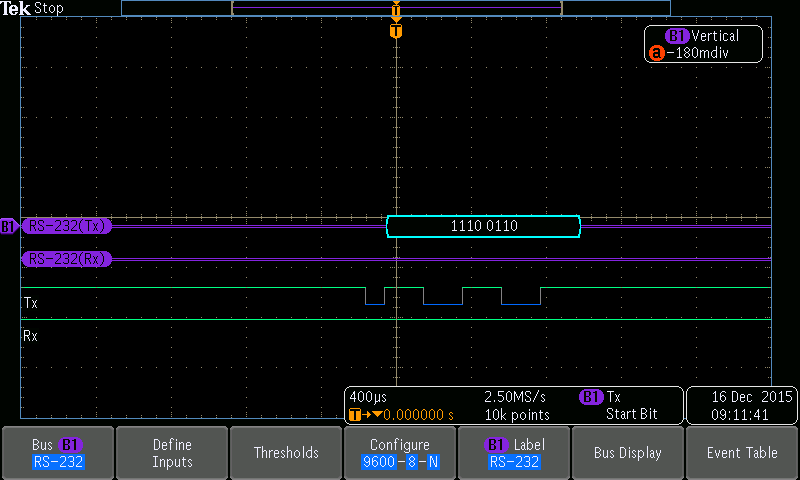
\includegraphics[scale=.75]{uart-message}
\\
Figure 1
\end {center}
2 h-bridge 2 speed, 2 h-bridge 2 speed



\begin {center}
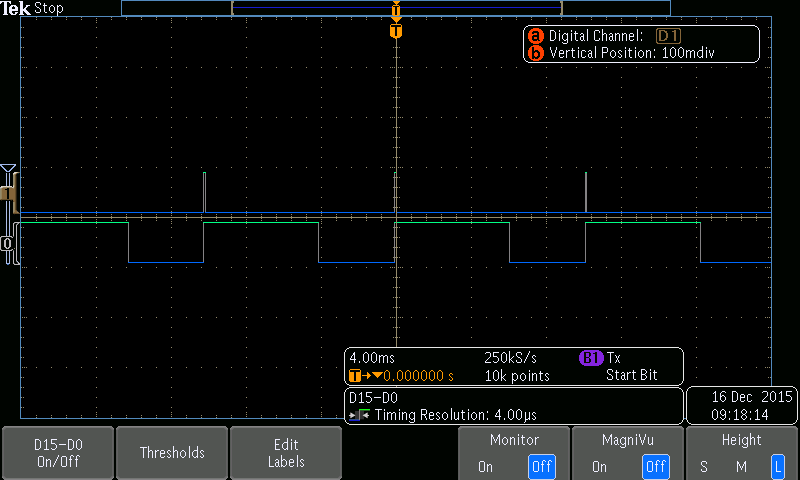
\includegraphics[scale=.75]{half-power}
\\
Figure 2
\end {center}
\begin {center}
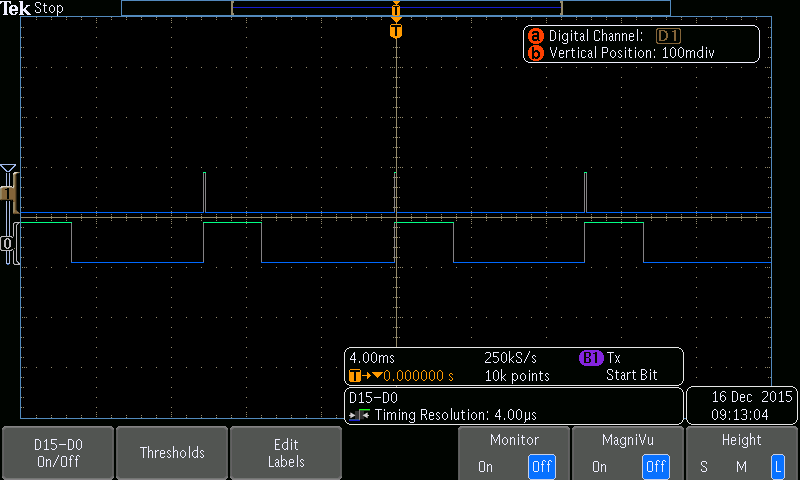
\includegraphics[scale=.75]{quarter-power}
\\
Figure 3
\end {center}

\newpage
\section{Code}
\begin{lstlisting}[language=c]
#include "GPIO.h"

volatile int UART2_NVIC_R __attribute__((at(0xE000E104)));

int PWM0Count = 0, PWM1Count = 0, PWM0Duty = 0, PWM1Duty = 0;
char turningRight = 0, turningLeft = 0;
char inData, hBridge1, hBridge2, drive1, drive2;


void PWM_init() {//page 1233
	SYSCTL_RCGC2_R |= 0x2;
	SYSCTL_RCGCPWM_R = 0x1;
	//enable PWM clock in RCGC0 register
	__nop();
	__nop();
	__nop();

	while((SYSCTL_PRGPIO_R&SYSCTL_PRGPIO_R1) == 0){};//wait for clock to stabilize

	//Setup GPIO port B
	GPIO_PORTB_LOCK_R = 0x4C4F434B;
	GPIO_PORTB_PUR_R = 0xC0;
	GPIO_PORTB_DIR_R = 0xC0;
	GPIO_PORTB_DEN_R = 0xC0;
}

void UART2_INIT() {
	//UART2 D6,D7
	SYSCTL_RCGCUART_R = 0x4;
	SYSCTL_RCGCGPIO_R |= 0x8;
	__nop();
	__nop();
	__nop();//clock needs some time to initialize
	GPIO_PORTD_LOCK_R = 0x4C4F434B;//unlock port c
	GPIO_PORTD_CR_R |= 0xC0;//enable control register,i dont think we need this
	GPIO_PORTD_AFSEL_R |= 0xC0;//alternative functionality enabled
	GPIO_PORTD_DEN_R |= 0xC0; //digital enable enabled
	GPIO_PORTD_PCTL_R = 0x11000000;//page 686 PD6 (1), PD7 (1)
	UART2_CTL_R = 0x0;//disable uart
	//(16e6)/(9600*16) = 104.167
	UART2_IBRD_R = 0x68;//104
	//.167 * 64 + .5 = 8.5 rounddown to 11 
	UART2_FBRD_R = 0xB;//11
	UART2_LCRH_R |= 0x72; //Set serial parameters: 8-bit word, start/stop/parity bits
	UART2_CTL_R = 0x301; // Enable rx, tx on uart
	//we can turn off tx if we can somehow link the phone
	//and bluetooth without needing to tx
	//INTERRUPT INIT for UART
	UART2_IFLS_R = 0x0;  //set interrupts rx 1/8 full queue 
	UART2_RIS_R = 0x10; //page 925
	UART2_IM_R  = 0x10; //interrupt mask, Rxim page 921
	UART2_NVIC_R = 0x2;
}

//Trigger when queue is 3/4 full(12 bytes)
void UART2_Handler() { 
	TIMER1_TAILR_R = 0x7A1200;       // Reset watchdog timer value    
	GPIO_PORTE_DATA_R = 0x0;         // Turn on headlights
	if((UART2_FR_R & 0x10) == 0x0) { // RxFE bit Read 1/8 full
		inData = UART2_DR_R;
	}

	//parse incoming data
	hBridge1 = inData & 0x3;
	drive1 = (inData & 0xC) >> 2;
	hBridge2 = (inData & 0x30) >> 4;
	drive2 = (inData & 0xC0) >> 6;

	//Only turn the drive motor if it is not on the stop
	if (hBridge1 == 0x1 && turningRight == 1) {
		hBridge1 = 0x11;
	}
	else if (hBridge1 == 0x10 && turningLeft == 1) {
		hBridge1 = 0x11;
	}
	
	// Write new command to gpio port
	GPIO_PORTA_DATA_R = (((hBridge1 << 2) | (hBridge2))<<4);
	PWM0Duty = drive1 * 30;
	PWM1Duty = drive2 * 30;

	UART2_ICR_R = 0x1;
}

//Systick initialization. Used for PWM output
void SystickConfig() {
	NVIC_ST_CTRL_R = 0;
	NVIC_ST_RELOAD_R = 0x640;
	NVIC_ST_CTRL_R = 0x7;
}

//Output PWM when systick expires
void SysTick_Handler(){
	PWM0Count++;
	PWM1Count++;

	if (PWM0Count > 100) {
		PWM0Count = 0;
	}

	if (PWM1Count > 100) {
		PWM1Count = 0;
	}

	if (PWM0Count > PWM0Duty) {
		GPIO_PORTB_DATA_R &= ~0x40;
	} 
	else {
		GPIO_PORTB_DATA_R |= 0x40;
	}

	if (PWM1Count > PWM1Duty) {
		GPIO_PORTB_DATA_R &= ~0x80;
	} 
	else {
		GPIO_PORTB_DATA_R |= 0x80;
	}

	NVIC_ST_CTRL_R = 0x7;
}

//Initialize port A, used for controlling the motors
void GPIOA_INIT() {
	//A2, A3, A4, A5, A6, A7
	SYSCTL_RCGC2_R |= 0x1;   //Enable clock for PortA
	GPIO_PORTA_DIR_R = 0xF0; //Set direction to output
	GPIO_PORTA_PUR_R = 0xC;  //Pull up resistor
	GPIO_PORTA_DEN_R = 0xFC; //Digitial enable
	GPIO_PORTA_IS_R = 0x1;   //Edge triggering
	GPIO_PORTA_IBE_R = 0x1;  //Trigger both edges
	GPIO_PORTA_IM_R = 0xC;   //Pin interrupt
	NVIC_EN0_R = 0x1;        //NVIC
}

//One of the interrupts from the turning feedback was triggered
void GPIOA_Handler() {
	char PORTA_DATA = GPIO_PORTA_DATA_R;
	//Check and see if it is turned to the right
	if ((PORTA_DATA & 0x8) != 0) {
		turningRight = 0;
		turningLeft = 1;
	}
	//Check and see if it is turned to the left
	else if ((PORTA_DATA & 0x4) != 0) {
		turningRight = 1;
		turningLeft = 0;
	}
	//Otherwise, somewhere in the middle
	else {
		turningRight = 0;
		turningLeft = 0;
	}

	GPIO_PORTA_ICR_R = 0xFF; //Service the interrupt
}

//Setup the GPIO port for the LED outptu (head and break lights)
void setupLED(){
	SYSCTL_RCGC2_R |= 0x10;  //Enable clock for PortE
	GPIO_PORTE_DIR_R = 0x1;  //set direction to output
	GPIO_PORTE_PUR_R = 0x1;  //Pull up resistor
	GPIO_PORTE_DEN_R = 0x1;  //digitial enable

	GPIO_PORTE_DATA_R = 0x1; //turn off LED lights
}

//Initialize timer 1, used as a watchdog
void Timer1A_init() {
	SYSCTL_RCGCTIMER_R = 0x2;
	TIMER1_CTL_R = 0x0;        //Stop timer
	TIMER1_CFG_R = 0x0;        //Select 32 bit mode
	TIMER1_TAMR_R = 0x2;       //Periodic mode
	TIMER1_TAILR_R = 0x7A1200; //Timer set to expire after 1 second
	TIMER1_IMR_R = 0x1;        //Enable interrupt on port
	NVIC_EN0_R |= (1 << 21);   //Enable in NVIC
	TIMER1_CTL_R = 0x1;        //Start timer
}

//Respond to the watchdog call
void TIMER1A_Handler() {
	TIMER1_ICR_R = 0x1F;
	GPIO_PORTE_DATA_R = 0x1;  //Turn off the lights
	GPIO_PORTA_DATA_R = 0xF0; //Stop the motors

	//Put the motors in stop mode
	PWM0Duty = 0;
	PWM1Duty = 0;
}

int main(void) {
	//Setup everything
	UART2_INIT();
	PWM_init();
	SystickConfig();
	GPIOA_INIT();
	setupLED();
	Timer1A_init();

	//Wait for bluetooth command
	while(1);
}
\end{lstlisting}

\end{document}